\documentclass[ignorenonframetext,8pt]{beamer}
\usepackage{graphicx}
\synctex=1
\usetheme{default}
\useoutertheme{infolines}

\useinnertheme{circles}
\usecolortheme{crane}

\usepackage[latin1]{inputenc}
\usepackage{helvet}
%\usepackage{uarial}

\usepackage{psfrag}
\usepackage{color, graphicx}
\usepackage{float}
\usepackage[italian]{babel}
\usepackage{hyperref}
\hypersetup{
    colorlinks,%
    citecolor=black,%
    filecolor=black,%
    linkcolor=black,%
    urlcolor=black
}
\setbeamerfont{frametitle}{size=\normalsize}
\setbeamerfont{frametitle}{series=\bfseries}
%\mode<presentation>


\author[Luigi Pasotti]{Candidato: Luigi Pasotti\\ Relatore: Prof. Alessandro Martinelli}
\title[Moduli per applicativi client-server SF]{Progetto di moduli per lo sviluppo di applicativi client-server basati su Shadow Framework}
\institute[Universit\`a di Pavia]{Universit\`a degli Studi di Pavia\\ Facolt\`a di Ingegneria\\ Dipartimento di Ingegneria Industriale e dell'Informazione}
\date[22/04/2013]{22 Aprile 2013}
%\logo{
\includegraphics[width=1cm]{Immagini/Unipv-logo-vett}}

\begin{document}
	\begin{frame}
		\begin{center}
			
\includegraphics[width=2cm]{Immagini/Unipv-logo-vett}
		\end{center}
		\titlepage
	\end{frame}

	\begin{frame}
		\frametitle{Contenuti della presentazione}
		\begin{block}
			\tableofcontents
		\end{block}
	\end{frame}

	\section{Introduzione}
	
	\subsection{Obbiettivo della tesi}
	\begin{frame}
		\frametitle{Obbiettivo della tesi}
		\begin{block}{Contesto}
			\begin{itemize}
				\item \textbf{Shadow Framework}: framework per la realizzazione di applicazioni che fanno uso di \textbf{grafica tridimensionale real-time} ideato e sviluppato dall'Ingegner Alessandro Martinelli
				\item Caratteristiche:
				\begin{itemize}
					\item \textbf{portabilit\`a}: scritto in Java (desktop, Android), versione C++ (desktop, iOS) in sviluppo % struttura, OpenGL es
					\item \textbf{design web-oriented}: in sviluppo una versione javascript % meccanismi
					\item \textbf{moderno}: massiccio utilizzo delle GPU a pipeline programmabile % caratteristiche avanzate delle API
					\item \textbf{estendibile}: uso di design pattern, modulare
				\end{itemize}
			\end{itemize}
		\end{block}

		\begin{block}{Obbiettivo}
			\begin{itemize}
				\item Produzione di moduli utili allo sviluppo di applicazioni client-server orientate al web:
				\begin{itemize}
					\item \textbf{estensione del layer dati}
					\item \textbf{dati grafici trasmessi in rete}
					%\item \textbf{modularit\`a}
				\end{itemize}
			\end{itemize}
		\end{block}
	\end{frame}

	\subsection{Web 3D e Tecnologie attuali}
	\begin{frame}
		\frametitle{Web 3D}
		\begin{block}{Fruizione tramite il web di contenuti in grafica 3D real-time interattiva}
			Applicazioni:
			\begin{itemize}
					\item navigazione web
					\item intrattenimento: giochi, social network
					\item eCommerce: vetrine interattive
			\end{itemize}
		\end{block}

		\begin{block}{Problematica}
			\begin{itemize}
					\item \textbf{dimensione dei dati} grafici non trascurabile (GigaByte)
			\end{itemize}
		\end{block}
	\end{frame}

	\begin{frame}
		\frametitle{Tecnologie Attuali}
		\begin{block}{Modalit\`a di fruizione usate da framework e applicazioni}
			\begin{itemize}
				\item \textbf{Plugin per browser}: Flash, Java, Ad hoc
				\item \textbf{WebGL}: javascript
				\item \textbf{Live streaming}: applicazioni native, Java Web Start, ecc.
			\end{itemize}
		\end{block}
		\begin{block}{Modalit\`a di trasmissione dati (e relativi problemi)}
			\begin{itemize}
				\item \textbf{Approccio stand-alone}: lunghi tempi di caricamento
				\item \textbf{Flusso continuo}: occupazione di banda
				\item \textbf{Trasferimento progressivo}: limitazioni alla qualit\`a dei dati
			\end{itemize}
		\end{block}
	\end{frame}

	\subsection{Shadow Framework}
	\begin{frame}
		\frametitle{Shadow Framework}
		\begin{block}{Focus sui 3 ``momenti'' di accesso ai dati grafici:}
			\begin{itemize}
				\item \textbf{Accesso}
				\item \textbf{Costruzione e Inizializzazione}
				\item \textbf{Visualizzazione}
			\end{itemize}
		\end{block}

		\begin{block}{Pipeline di accesso ai dati}
			\begin{center}
				\only<1>{\textbf{Approccio classico (tipo stand-alone)}}
				\only<2>{\textbf{Approccio live streaming}}
				\only<3>{\textbf{Approccio SF}}

				\includegraphics<1>[width=.70\textwidth]{Immagini/classicdecompressionpipeline}
				\includegraphics<2>[width=.70\textwidth]{Immagini/streamingdecompressionpipeline}
				\includegraphics<3>[width=.70\textwidth]{Immagini/sfdecompressionpipeline}
			\end{center}
		\end{block}
	\end{frame}

	\begin{frame}
		\frametitle{Confronto rappresentazione dati}
		\begin{block}{Rendering della stessa geometria in \textbf{formato SF} (sinistra) ed in forma di \textbf{mesh poligonale} (destra)}
			\begin{center}
				\begin{minipage}[c]{.45\textwidth}
					\begin{figure}
						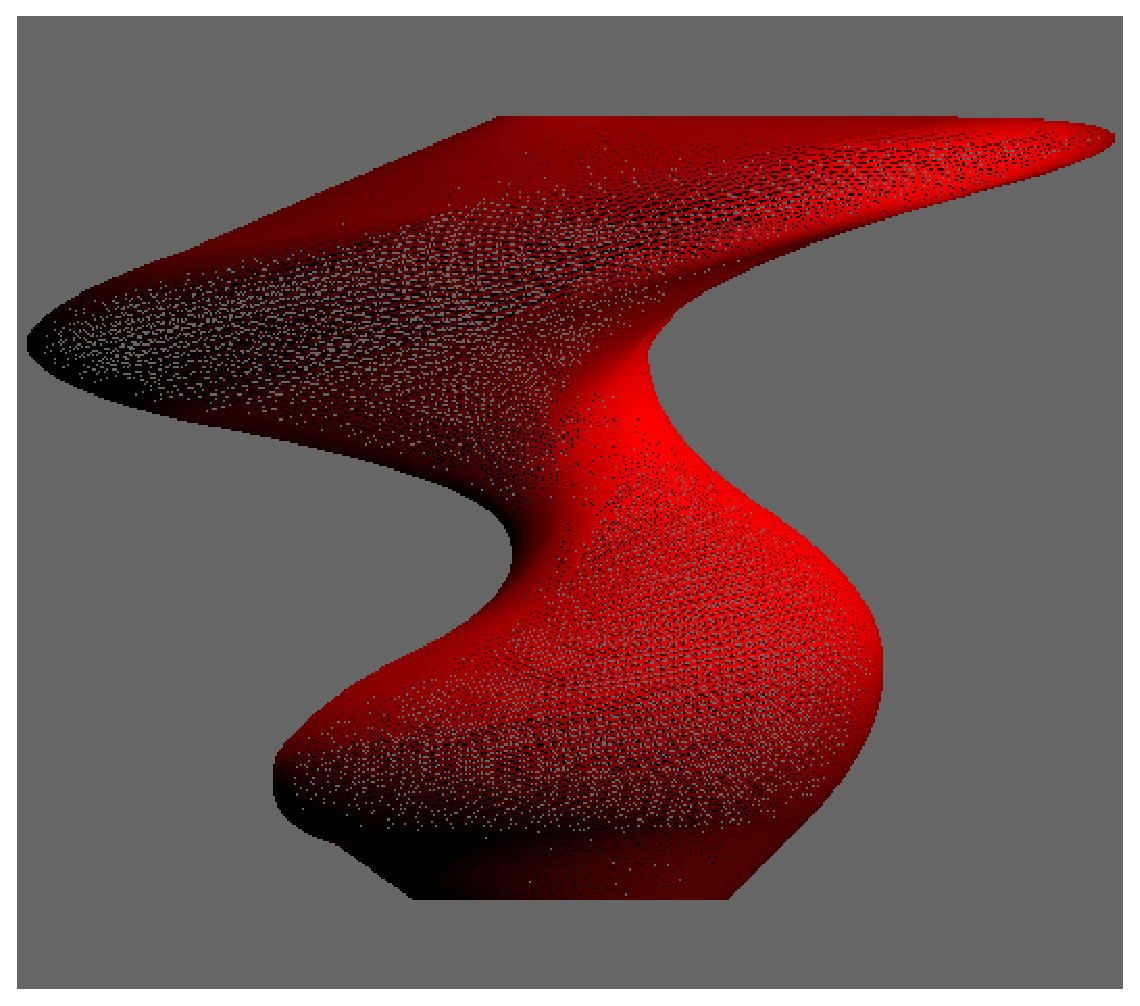
\includegraphics[width=\textwidth]{Immagini/fungoSF}
					\end{figure}
				\end{minipage}
				\begin{minipage}[c]{.45\textwidth}
					\begin{figure}
						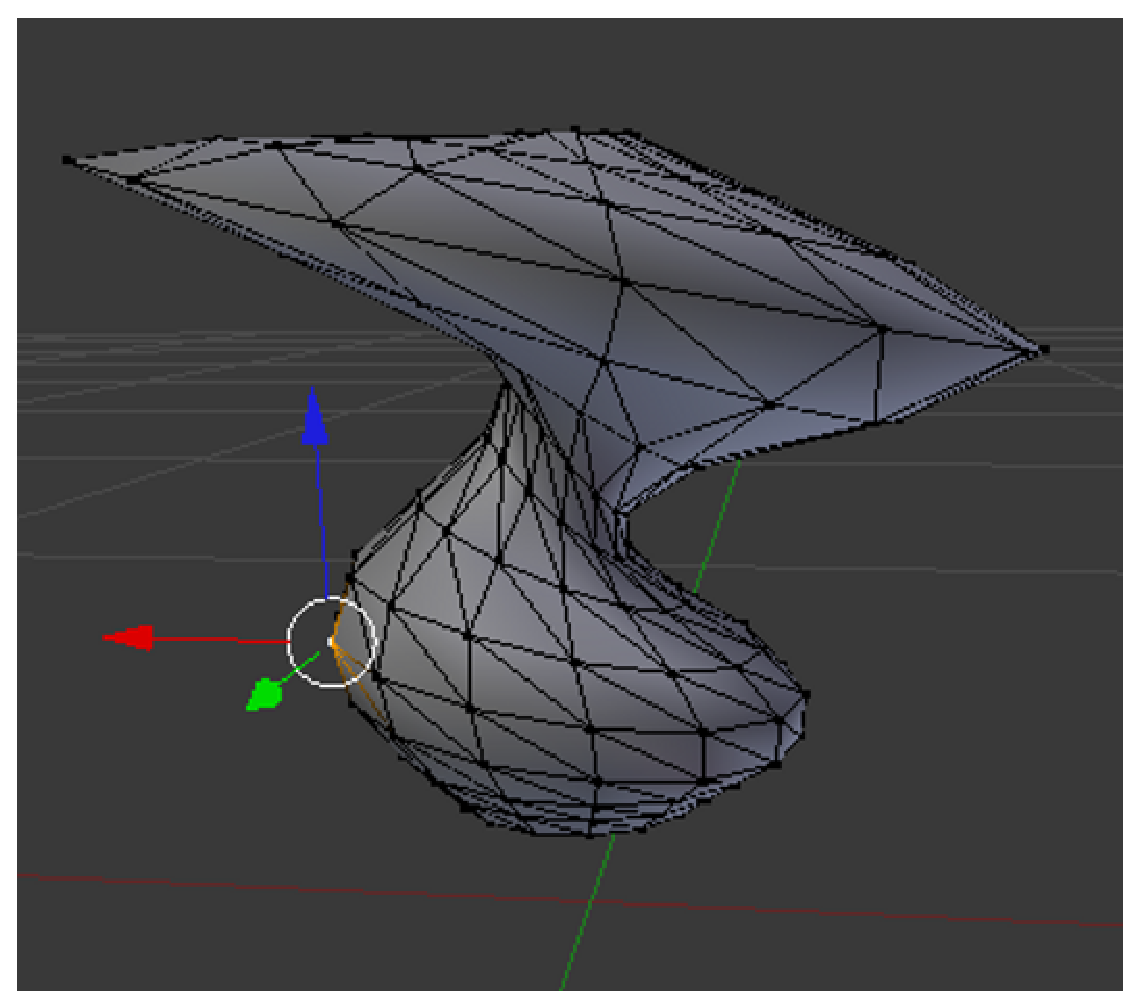
\includegraphics[width=\textwidth]{Immagini/fungoObj}
					\end{figure}
				\end{minipage}
			\end{center}
			\begin{center}
				\begin{minipage}[c]{.45\textwidth}
					%\footnotesize 
					\begin{itemize}
						\item dimensione xml: \textbf{3 kB}
						\item dimensione file .sf: \textbf{263 Byte}
						\item dimensione file .sf (con sola geometria): \textbf{64 Byte}
					\end{itemize}
				\end{minipage}
				\begin{minipage}[c]{.45\textwidth}
					%\footnotesize 
					\begin{itemize}
						\item dimensione Collada: \textbf{55,3 kB} (standard xml riconosciuto)
						\item dimensione obj: \textbf{34,3 kB}
						\item dimensione file .3ds: \textbf{8,6 kB}
					\end{itemize}
				\end{minipage}
			\end{center}
		\end{block}
	\end{frame}

	%\subsection{Layer Dati Shadow Framework}
	\begin{frame}
		\frametitle{Layer Dati Shadow Framework}
		\begin{block}{Dati gestiti tramite astrazione}
			\begin{itemize}
				\item \textbf{SFDataset}: unit\`a base di ogni dato del framework
				\item \textbf{SFDataCenter}: gestore centralizzato dei dati
					\begin{itemize}
						\item \textit{Singleton}
						\item \textit{Bridge}
					\end{itemize}
			\end{itemize}
			\begin{figure}
				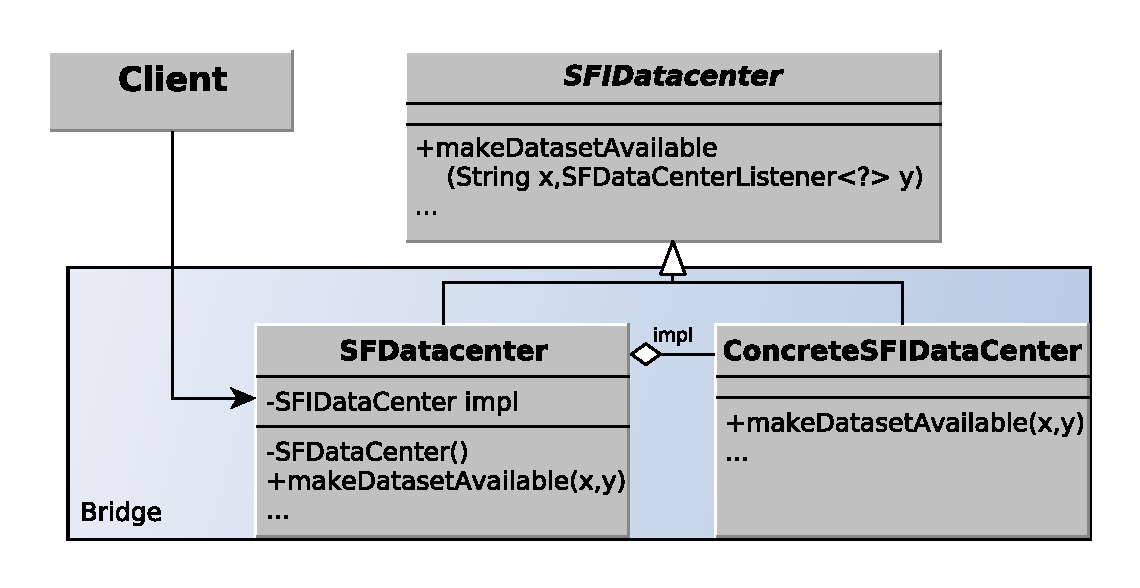
\includegraphics[width=.70\textwidth]{Immagini/DataCenter}
			\end{figure}
		\end{block}
	\end{frame}

	\section{SF-Remote-Connection}

	\begin{frame}
		\frametitle{SF-Remote-Connection}
		\begin{block}{Moduli del progetto}
			\begin{itemize}
				\item \textbf{Base Communication}
					\begin{itemize}
						\item Libreria per comunicazione via TCP
					\end{itemize}
				\item \textbf{RemoteDataCenter Tool}
					\begin{itemize}
						\item Implementazione di \textit{SFIDataCenter} che usa la comunicazione di rete
					\end{itemize}
				\item \textbf{Client}
					\begin{itemize}
						\item Libreria per applicazioni client
					\end{itemize}
				\item \textbf{Server}
					\begin{itemize}
						\item Libreria per applicazioni server
					\end{itemize}
			\end{itemize}
		\end{block}
	\end{frame}
	
	\subsection{Moduli}
	%\subsection{Base Communication}
	\begin{frame}
		\frametitle{Base Communication}
		\framesubtitle{Libreria per comunicazione via TCP}
		\begin{block}{Caratteristiche salienti}
			\begin{itemize}
				\item Gestione connessioni client e server
				\item Scambio messaggi testuali via TCP
				\item \textbf{Configurabilit\`a} protocollo di comunicazione attraverso il \textbf{pattern \textit{State}}
			\end{itemize}
			\begin{figure}
				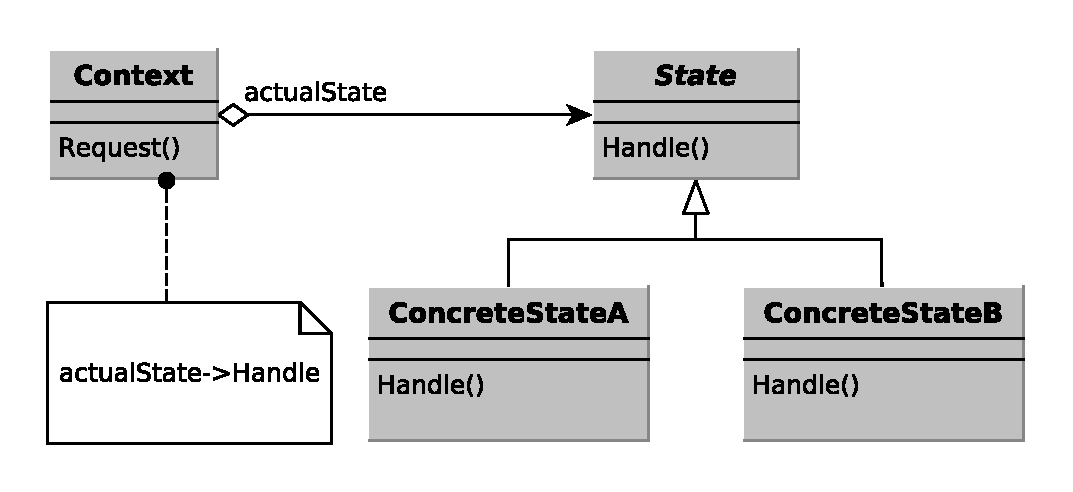
\includegraphics[width=.70\textwidth]{Immagini/StatePattern}
			\end{figure}
		\end{block}
	\end{frame}

	%\subsection{RemoteDataCenter Tool}
	\begin{frame}
		\frametitle{RemoteDataCenter Tool}
		\framesubtitle{Implementazione di \textit{SFIDataCenter} che usa la comunicazione di rete}
		\begin{block}{Caratteristiche salienti}
			\begin{itemize}
				\item \textbf{Coda di richieste}
				\item Meccanismo a \textbf{Dataset sostitutivi}
			\end{itemize}
			\begin{figure}
				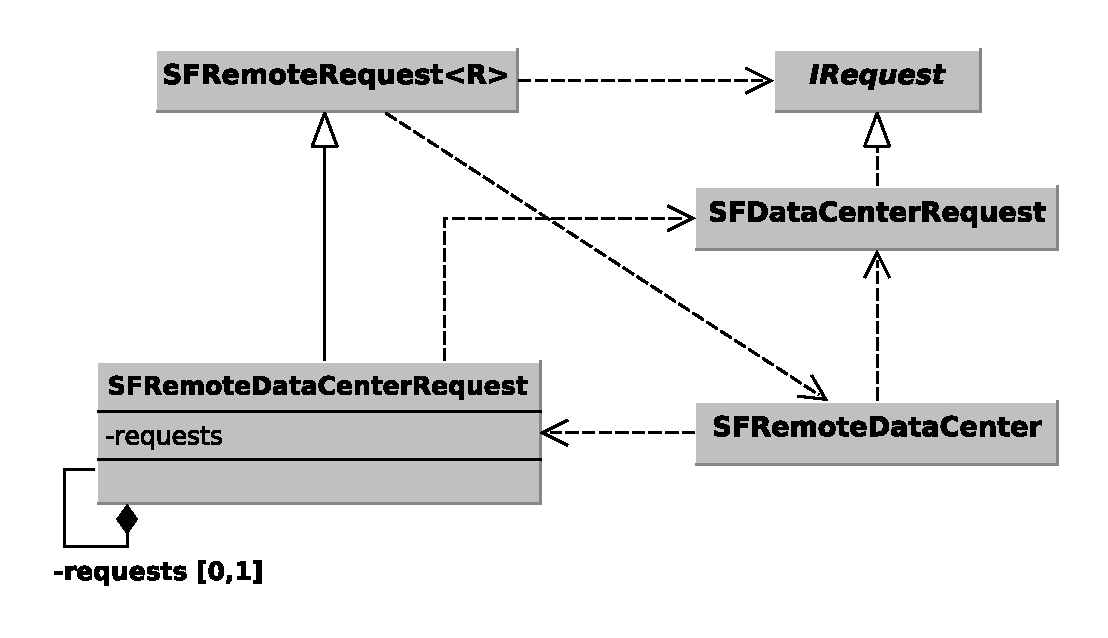
\includegraphics[width=.60\textwidth]{Immagini/RemoteDataCenter}
			\end{figure}
		\end{block}
	\end{frame}

	%\subsection{Client}
	\begin{frame}
		\frametitle{Client}
		\framesubtitle{Libreria per applicazioni client}
		\begin{block}{Caratteristiche salienti}
			\begin{minipage}[c]{.40\textwidth}
				\begin{itemize}
					\item Implementazione del reperimento dati
						\begin{itemize}
							\item \textbf{Bufferizzazione} delle richieste
							\item \textbf{Multithread}
						\end{itemize}
					\item Macchina a stati per la gestione del protocollo lato client
						\begin{itemize}
							\item \textbf{Espandibilit\`a}
							\item \textbf{Test-oriented}
						\end{itemize}
				\end{itemize}
			\end{minipage}
			\begin{minipage}[c]{.59\textwidth}
				\begin{figure}
					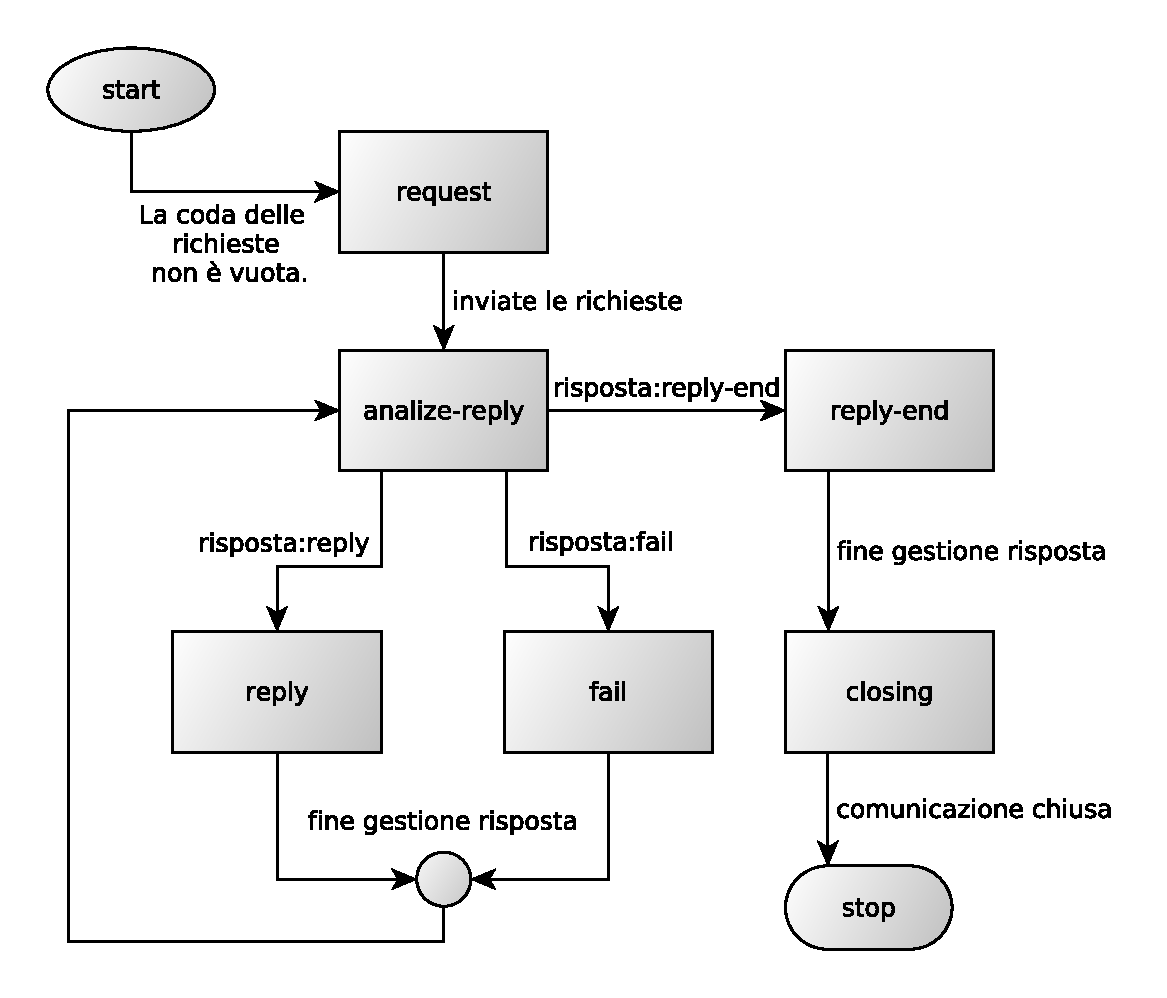
\includegraphics[width=\textwidth]{Immagini/StateMachineClient}
				\end{figure}
			\end{minipage}
		\end{block}
	\end{frame}

	%\subsection{Server}
	\begin{frame}
		\frametitle{Server}
		\framesubtitle{Libreria per applicazioni server}
		\begin{block}{Caratteristiche salienti}
			\begin{minipage}[c]{.49\textwidth}
				\begin{itemize}
					\item \textbf{No stack grafico}, solo gestione dei dati
					\item \textbf{Multithread}
					\item Macchina a stati per la gestione del protocollo lato server
						\begin{itemize}
							\item \textbf{Espandibilit\`a}
							\item \textbf{Test-oriented}
						\end{itemize}
				\end{itemize}
			\end{minipage}
			\begin{minipage}[c]{.50\textwidth}
				\begin{figure}
					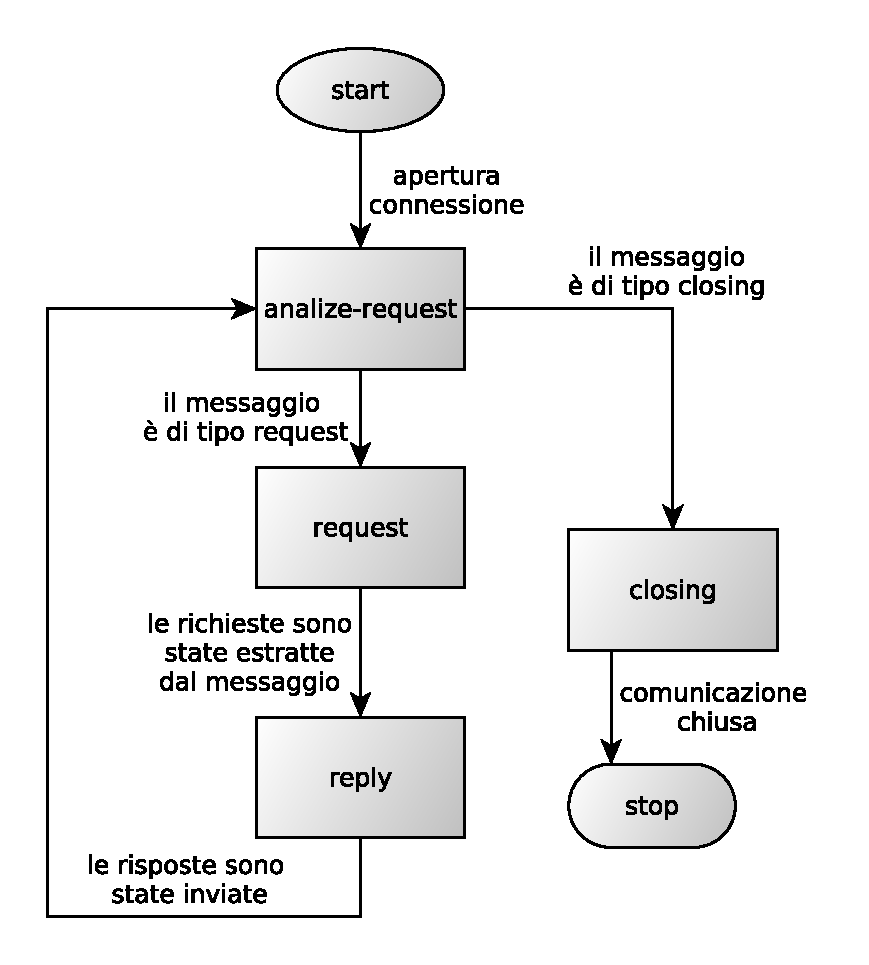
\includegraphics[width=\textwidth]{Immagini/StateMachineServer}
				\end{figure}
			\end{minipage}
		\end{block}
	\end{frame}

	\subsection{Dataset sostitutivi}
	\begin{frame}
		\frametitle{Dataset sostitutivi}
		\begin{onlyenv}<1-2>
			\begin{block}{Motivazioni}
				\begin{itemize}
					\item Reperimento dati non bloccante
					\item Possibilit\`a di definire dei ``segna-posto'' per gli elementi grafici
				\end{itemize}
			\end{block}
			\begin{center}
				\begin{figure}
					\includegraphics<1>[width=.90\textwidth]{Immagini/sequenzaDatiSost}
					\includegraphics<2>[width=.90\textwidth]{Immagini/sequenzaDatiSost2}
				\end{figure}
			\end{center}
		\end{onlyenv}
		\begin{onlyenv}<3>
			\begin{block}{Update dei dati}
				\begin{itemize}
					\item Deve affrontare la \textbf{costruzione e inizializzazione} dei dati ricevuti
					\item Deve essere sincronizzato con il processo di rendering:
						\begin{itemize}
							\item meccanismo interno al framework che usa un Updater e un Initiator.
						\end{itemize}
				\end{itemize}
			\end{block}
			\begin{center}
				\begin{figure}
					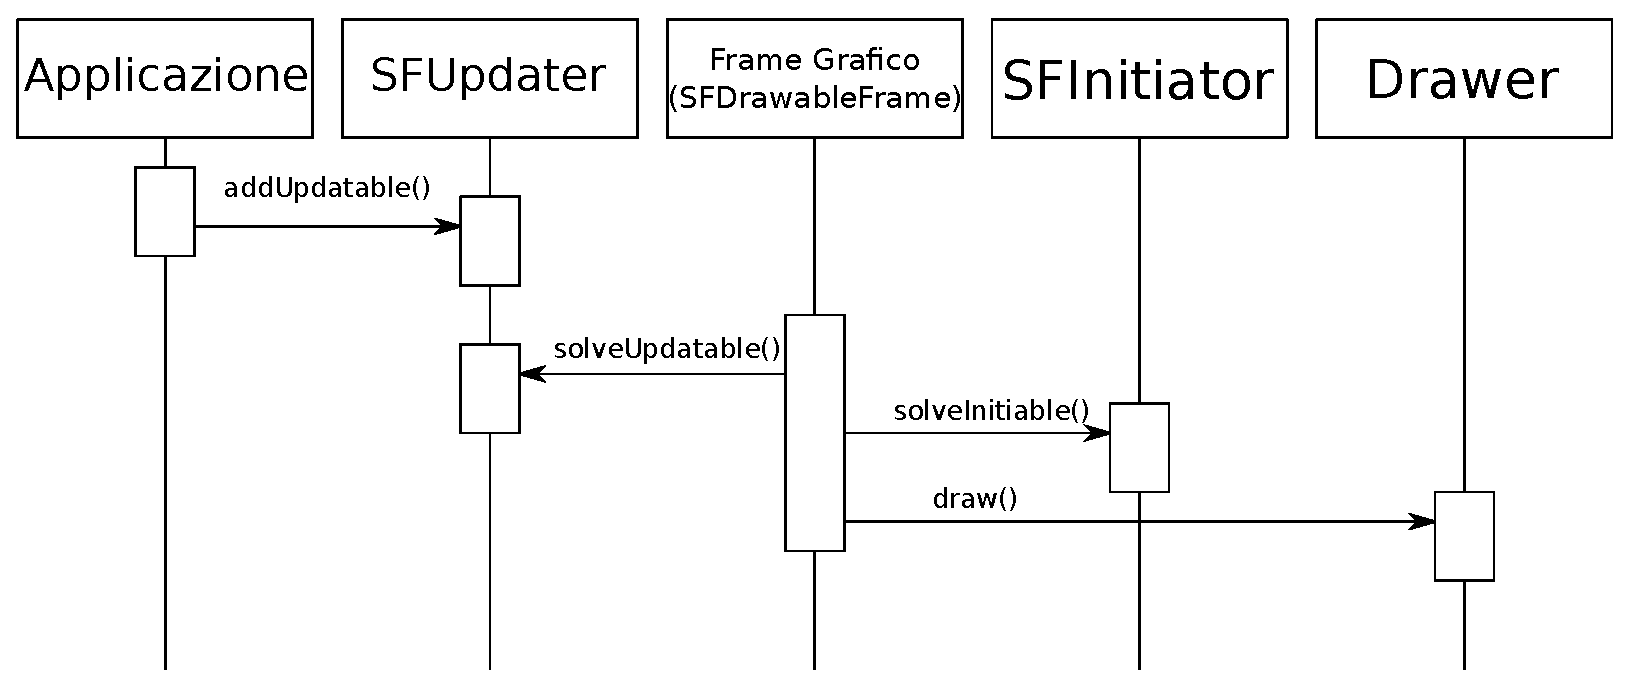
\includegraphics[width=.80\textwidth]{Immagini/sequenzaUpdatable}
				\end{figure}
			\end{center}
		\end{onlyenv}
	\end{frame}

	% \begin{frame}
	% 	\frametitle{Comunicazione}
	% 	\begin{block}
			
	% 	\end{block}
	% \end{frame}

	\section{Test}

	\begin{frame}
		\frametitle{Test}
		\begin{block}{Test dal vivo}
			\begin{center}
				Buona visione
			\end{center}
		\end{block}
	\end{frame}

	\section{Risultati e sviluppi futuri}

	\begin{frame}
		\frametitle{Conclusioni}
		\begin{block}{Conclusioni}
			\begin{itemize}
					\item I moduli:
						\begin{itemize}
							\item rispecchiano le caratteristiche volute;
							\item sono facilmente \textbf{estendibili}.
						\end{itemize}
					\item Acquisita familiarit\`a con pratiche e tecniche riconosciute:
						\begin{itemize}
							\item uso di \textbf{Design Pattern};
							\item metodi di \textbf{sviluppo agile};
							\item strumenti di \textbf{controllo di versione concorrente}.
						\end{itemize}
					\item Importante \textbf{feedback} sulle componenti interne dello Shadow Framework
			\end{itemize}
		\end{block}
		\begin{block}{Sviluppi futuri}
			\begin{itemize}
				\item Strumenti per una comunicazione pi\`u complessa
				\item Tool per la definizione dei Dataset sostitutivi
				\item Invio di Dataset aggregati in librerie
			\end{itemize}
		\end{block}
	\end{frame}

	\begin{frame}
		\begin{center}
			
\includegraphics[width=2cm]{Immagini/Unipv-logo-vett}
		\end{center}
		\titlepage
	\end{frame}
\end{document}